Aujourd'hui, tous les ordinateurs grand public ont une interface graphique, qu'on pilote principalement avec la souris; le clavier ne sert plus qu'à taper du texte. Cependant, il n'en a pas toujours été ainsi! Au début de l'informatique, toutes les interactions se faisaient au clavier, dans ce qu'on appelle la \textbf{console}, ou \textbf{terminal} (figure \ref{terminal}).

\begin{figure}[h!]
\begin{center}
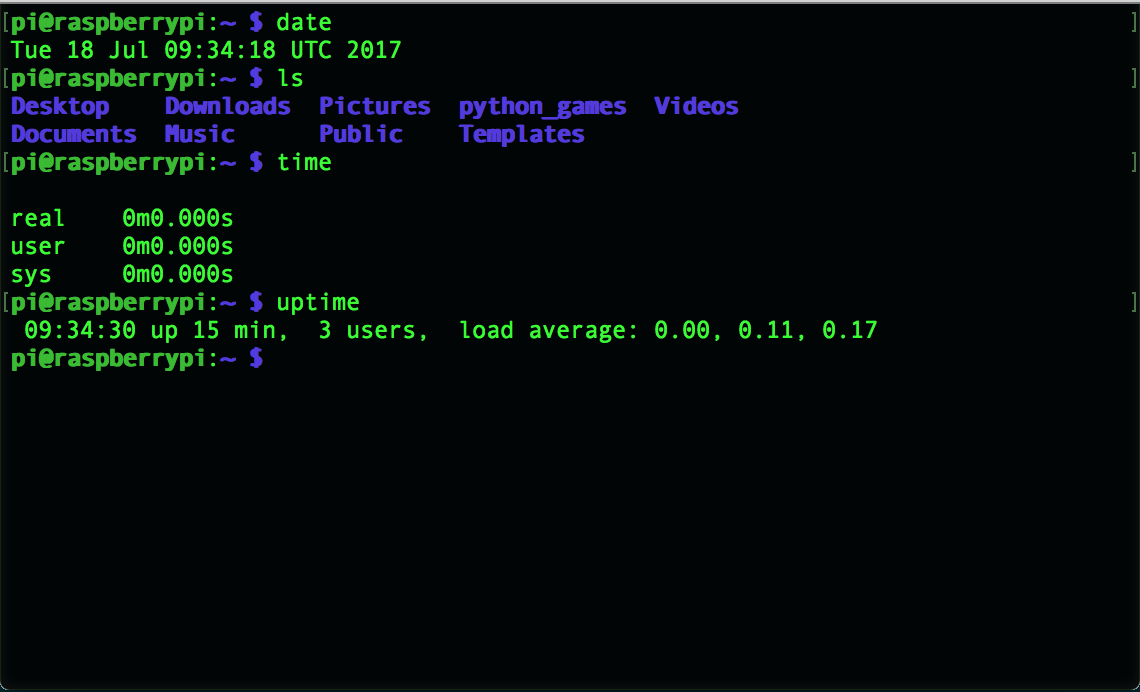
\includegraphics[width=10cm]{ssh.png}
\end{center}
\caption{Le terminal}
\label{terminal}
\end{figure}

Bien que sur Windows ou macOS, on n'utilise presque plus le terminal, il a encore une certaine utilité sur les distributions Linux, dont Raspbian fait partie.
Il existe des commandes très pratiques pour rapidement mettre à jour ses programmes, ou bien configurer certains aspects du Raspberry Pi.

On accède au terminal du Raspberry Pi en appuyant sur la quatrième icône de la barre des menus (voir figure \ref{interface}).